% !TEX encoding = UTF-8 Unicode
\documentclass{article}           % use "amsart" instead of "article" for AMSLaTeX format
\usepackage{geometry}                           % See geometry.pdf to learn the layout options. There are lots.
\geometry{letterpaper}                          % ... or a4paper or a5paper or ... 
%\geometry{landscape}                           % Activate for for rotated page geometry
%\usepackage[parfill]{parskip}                  % Activate to begin paragraphs with an empty line rather than an indent
\usepackage{graphicx}                           % Use pdf, png, jpg, or eps§ with pdflatex; use eps in DVI mode
                                                % TeX will automatically convert eps --> pdf in pdflatex                

\usepackage[utf8]{inputenc}
\usepackage[T1]{fontenc}

\usepackage{amssymb}
\usepackage{amsmath}
\usepackage{amsthm}

\usepackage{caption}
\usepackage{subcaption}

\usepackage{tikz}
\usetikzlibrary{arrows}
\usetikzlibrary{shapes, arrows.meta}

\usepackage{../tex/mathpartir}
\usepackage{url}

\newtheorem{definition}{Definition}
\newtheorem{lemma}{Lemma}
\newtheorem{theorem}{Theorem}
\newtheorem{corrolary}{Corrolary}
\newtheorem{claim}{Claim}
 
\newcommand{\R}{\mathbb{R}}
\newcommand{\cov}{\vartriangleleft}
\newcommand{\Pos}{\mathsf{Pos}}
\newcommand{\List}[1]{\mathsf{List}\ {#1}}
\newcommand{\fun}[2]{\lambda {#1}.\  {#2}}
\newcommand{\nat}{\mathbb{N}}
\newcommand{\rat}{\mathbb{Q}}
\newcommand{\suchthat}{\ |\ }
\newcommand{\concat}{\ensuremath{+\!\!\!\!+\,}}
\newcommand{\One}{\mathsf{One}}
\newcommand{\Dist}[1]{\mathcal{M}({#1})}
\newcommand{\Open}[1]{\mathcal{O}({#1})}
\newcommand{\coinflip}{\mathsf{coinflip}}
\newcommand{\Sampler}{\mathsf{Sampler}}
\newcommand{\bool}{\mathbb{B}}
\newcommand{\cons}{::}
\newcommand{\un}[1]{\ \mathrm{#1}}
\newcommand{\irule}[1]{\textsc{#1}}
\newcommand{\Type}{\mathcal{U}}
\newcommand{\Prop}{\mathcal{P}}

\newcommand{\Space}{\mathsf{Space}}
\newcommand{\Prob}{\mathcal{P}}
\newcommand{\PLower}{\mathcal{L}^+}
\newcommand{\Viet}{{\mathcal{V}^+}}

\newcommand{\map}[1]{\mathsf{map}_{#1}}
\newcommand{\ret}[1]{\mathsf{ret}_{#1}}
\newcommand{\join}[1]{\mathsf{join}_{#1}}
\newcommand{\ratint}{\rat_\mathbb{I}}

\newcommand{\HeineBorel}{\mathsf{HB}}

\newcommand{\lowerT}[1]{\overrightarrow{#1}}
\newcommand{\upperT}[1]{\overleftarrow{#1}}
%\newcommand{\lowerT}[1]{\uparrow {#1}}

\newcommand{\truncate}[1]{\mathsf{trunc}\left({#1}\right)}

\newcommand{\dirsup}{\mathop{\setlength{\unitlength}{.7em}\raisebox{-.2em}%
    {\begin{picture}(1,1.5)\put(.5,0){\line(-1,3){.48}}
    \put(.5,0){\vector(1,3){.5}}\end{picture}}}} 
    
\newcommand{\ve}[1]{\mathbf{#1}}

\newcommand{\then}{\ ;\ }

\newcommand{\defeq}{\triangleq}

\title{Applications of formal topology}
\author{Ben Sherman}
%\date{\today}                                  % Activate to display a given date or no date

\begin{document}
\maketitle

What are potential applications of my framework for formal topology?

\section{The powerspaces: reasoning with and simulating uncertainty}

\subsubsection{Introduction}

Why do we need a new programming language where types are topological spaces and expressions are continuous maps? After all, if one programs in Martin-Löf type theory (without axioms), then, as Escardó says \cite{escardo4wft}, ``Secretly, types are \emph{spaces} and functions are \emph{continuous}.''

The issue is that this fact is a metatheorem, and so one cannot intrinsically reason about topology within Martin-Löf type theory. Or at the very least, the topology is necessarily very sensitive to which axioms are employed. In particular, the existence of type whose topology as a space is not discrete is incompatible with the law of the excluded middle (LEM). So if one really wishes to reason about this ``intrinsic'' topology in Martin-Löf type theory, one must necessarily employ anti-classical axioms (i.e., axioms which violate LEM). One such axiom is Brouwer's continuity principle, which says that all functions on the Baire space ($\nat \to \nat$) are (pointwise) continuous:\footnote{The $\exists$ quantifier must be interpreted as ``mere'' existence or truncated existence, or it is not consistent\cite{escardo2015inconsistency}.}
\[
\forall f : (\nat \to \nat) \to \nat, 
\forall \alpha : \nat \to \nat,
\exists n : \nat,
\forall \beta : \nat \to \nat,
\alpha =_n \beta
\to
f \alpha = f \beta,
\]
where $\alpha =_n \beta$ means that the sequences $\alpha$ and $\beta$ agree on the first $n$ values.

A similar axiom is the uniform continuity principle, which states that all functions on the Cantor space ($\nat \to \bool$) are uniformly continuous:
\[
\forall f : (\nat \to \bool) \to \bool,
\exists n : \nat,
\forall \alpha, \beta : \nat \to \bool,
\alpha =_n \beta
\to
f \alpha = f \beta.
\]

An issue with adding these axioms (other than violating LEM, which seems to make people uncomfortable) is that they don't have any computational interpretation, so it is impossible to program using them.

My goal, with my programming language for formal topology, is to create a world where types are spaces, and expressions are continuous maps, and it is no secret! Making the topological nature of the programming language overt\footnote{No pun intended.}, and computable, has several advantages. Not only does it provide an alternative way to think about writing programs, but it also opens up new computational and reasoning possibilities that are not available with Martin-Löf type theory with its ``intrinsic topology.''

This article explore how these newfound capabilities manifest with ``powerspaces'', topological spaces whose points are in some sense collections of points of another topological space. If we let $\Space$ denote the type of topological spaces, then the powerspaces have type $\Space \to \Space$. In particular, they are monads. It will focus on two specific powerspaces: the inhabited Vietoris powerspace $\Viet$\footnote{Paul Taylor calls this property \emph{supported} rather than \emph{inhabited}, because he takes ``inhabited'' to mean that the space has points, and rightly points out that there could be a nontrivial space $A$ which has no points, in which one might want to consider the powerspace $\Viet(A)$, as opposed to the $\mathcal{V}(A)$, even though $\Viet(A)$ will have no points as well.}, and the probabilistic powerspace $\Prob$.

With these powerspaces, it is possible to both \emph{compute} with and \emph{reason} about non-determinism. The inhabited Vietoris powerspace represents demonic and angelic nondeterminism, while the probabilistic powerspace represents probabilistic non-determinism. In particular, we can lift  computation $f : A_1 \times \cdots \times A_n \to B$ defined on points to the lifted computation $f_\Viet : \Viet(A_1) \times \cdots \times \Viet(A_n) \to \Viet(B)$ which tracks how angelic/demonic uncertainty in inputs affects the output, or similarly, a lifted computation $f_\Prob : \Prob(A_1) \times \cdots \times \Prob(A_n) \to \Prob(B)$ which tracks how (independent) probabilistic uncertainty in inputs results in a probabilistically uncertain output. The ability to define these lifted computations is a straightforward consequence of the monadicity of $\Viet$ and $\Prob$.

\subsubsection{An example task}

Let's be more concrete. We consider the following task from the Uncertain<T> paper \cite{uncertaint}. Somebody is walking with their mobile phone, which has a GPS device. Periodically, the phone polls the GPS and estimate's the user's walking speed. If we think that the user is walking faster than 4 mph, we'd like to sound an alarm to warn the user to slow down, but we'd prefer false negatives (the user is walking faster than 4mph but we don't catch it) to false positives (the user is walking slower than 4mph but we sound the alarm).

The naïve approach this program simply takes point estimates from the GPS and computes the speed with those coordinates, and checks whether it is larger than 4mph to determine whether to alarm the user. We can think of this computation as a function which takes the two position coordinates whose time difference is $\Delta t > 0$ as input and estimates the speed accordingly:
\begin{align*}
\mathsf{compute\_speed} : \R^2 \times \R^2 &\to \R
\\ \mathsf{compute\_speed} (x_1, y_1) (x_2, y_2) &= \frac{1}{\Delta t} \sqrt{(x_2 - x_1)^2 + (y_2 - y_1)^2}.
\end{align*}
As \cite{uncertaint} points out, this fails to account for the uncertainty in the GPS position estimates, an in particular we are likely to overestimate the user's speed with this strategy, and alarm the user much too frequently.

We can model the error in GPS coordinates in two ways: with (worst-case) non-determinism or with probabilistic non-determinism. The simpler one is the worst-case non-determinism. For instance, we imagine that there was a real position $\ve{x}$ obscured with some additive noise $\ve{n}$ such that the magnitude of the noise is not too large, i.e., $\| \ve{n} \| \le \varepsilon$ for some $\varepsilon \ge 0$.

By modeling such non-determinism with the Vietoris powerspace, we can automatically lift the $\mathsf{compute\_speed}$ map to one that operates on uncertain positions to produce an uncertain speed estimate. Then, instead of asking the question whether our speed estimate is greater than 4mph, we can ask: Is the speed \emph{necessarily} greater than 4mph? Is the speed \emph{possibly} greater than 4mph? We can \emph{compute} the answer to these questions, in a strong sense, as we could compute whether a single speed estimate is greater than 4mph.

The second way to take into account the uncertainty of the GPS estimates, which is probably more appropriate in this case, is to model the GPS estimates as corrupted with a probabilistic noise. So our real position $\ve{x}$ is obscured with additive noise $\ve{n}$ which is drawn from a normal distribution with mean 0 and variance $\sigma^2$. Now, for each real number $p : \R$ such that $0 \le p < 1$, we can ask whether the probability that the speed is greater than 4mph is greater than $p$, and again, this is computable in the same sense as the previous analogous questions.

The remainder of this article will give a vague and incomplete explanation of how formal topology works, how the powerspaces are defined, and how we can solve the above task with formal topology.

\subsubsection{A taste of formal topology}

In the constructive formulation of topological spaces, spaces are just logical theories in a restricted fragment of logic known as \emph{propositional geometric logic}. In this fragment of logic, we are only allowed to use finite conjunctions and infinitary disjunctions; no implication or negation. The formulae in these theories represent \emph{observable} properties of a space. They are also called \emph{opens}, because they represent what would be the open sets in conventional topology. For instance, the real numbers $\R : \Space$ are defined by the theory with atomic propositions $a < \cdot < b$ for each $a, b : \rat$ such that $a < b$, which are just syntactic objects which represent the proposition that a real number is greater than $a$ and less than $b$. The theory then has the following axioms which relate the propositions:

\begin{figure}[h!]
\caption{Logic of observables for $\R$.}
\label{Rcov}
\begin{center}
\begin{subfigure}[t]{0.4\textwidth}
\begin{center}
 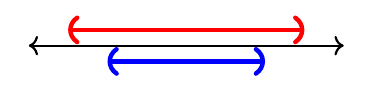
\begin{tikzpicture}
 \draw [<->, thick] (-2, 0) -- (2, 0);
 \draw [(-), ultra thick, blue] (-1, -0.2) -- (1, -0.2);
 \draw [(-), ultra thick, red] (-1.5, 0.2) -- (1.5, 0.2);
 \end{tikzpicture}
 \end{center}
\begin{mathpar}
\inferrule* [right=widen]
  {p' \le p < q \le q' }
  {p < \cdot < q \vdash p' < \cdot < q'}
\end{mathpar}
\end{subfigure}
~
\begin{subfigure}[t]{0.4\textwidth}
\begin{center}
 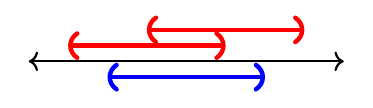
\begin{tikzpicture}
 \draw [<->, thick] (-2, 0) -- (2, 0);
 \draw [(-), ultra thick, blue] (-1, -0.2) -- (1, -0.2);
 \draw [(-), ultra thick, red] (-1.5, 0.2) -- (0.5, 0.2);
  \draw [(-), ultra thick, red] (-0.5, 0.4) -- (1.5, 0.4);
 \end{tikzpicture}
 \end{center}
\begin{mathpar}
\inferrule* [right=split]
  {r < p < u < s < q < v}
  {p < \cdot < q \vdash r < \cdot < s \ \vee\  u < \cdot < v }
\end{mathpar}
\end{subfigure}

\vspace{1em}

\begin{subfigure}[t]{0.4\textwidth}
\begin{center}
 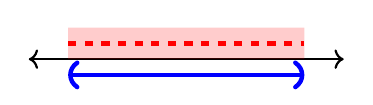
\begin{tikzpicture}
 \draw [<->, thick] (-2, 0) -- (2, 0);
 \draw [(-), ultra thick, blue] (-1.5, -0.2) -- (1.5, -0.2);
 \draw [ultra thick, dashed, red] (-1.5, 0.2) -- (1.5, 0.2);
  \fill[fill=red, opacity=0.2]  (-1.5, 0)--(-1.5,0.4)--(1.5,0.4)--(1.5,0)--(-1.5,0);
 \end{tikzpicture}
 \end{center}
\begin{mathpar}
\inferrule* [right=inside]
  { }
  {p < \cdot < q \vdash \bigvee \{ x < \cdot < y \suchthat p < x < y < q \}}
\end{mathpar}
\end{subfigure}

\end{center}
\end{figure}

The opens are observable, in the sense that if it is a theorem for a space that some (possibly infinitary) disjunction holds, i.e.,
\[
\top \vdash \bigvee_{i : I} P(i),
\]
then a point of a space can \emph{compute} some proposition of that disjunction which holds of that particular point. Said in a more spatial language, the above theorem represents an open cover of a space, and a point can \emph{compute} for any such open cover an open set of that cover which it lies in. A point is defined by the observable propositions that hold of it, i.e., the opens that it lies in. For a point $x : \R$ and open $P : \Open{\R}$, we write $x \models P$ (read ``$x$ lies in $P$'') if the property $P$ holds of $x$. Then we formally state the previously mentioned computation rule for points as \footnote{We assume that we are working in a constructive metatheory, and read the existential in the conclusion of \irule{split-cov} as constructive. That is, from the data in the hypothesis, one can compute the index $i : I$ of the disjunct which holds.}
\begin{mathpar}
\inferrule* [right=split-cov]
  {x \models P \qquad P \vdash \bigvee_{i : I} Q(i)}
  {\exists i : I, x \models Q(i) }
\end{mathpar}

We write $\Open{\R}$ to represent the opens of $\R$, so for any $a, b : \rat$ we have $a < \cdot < b : \Open{\R}$. It turns out that we can represent opens also as continuous maps from the space of interest to the Sierpínski space $\Sigma$, and it's convenient to conflate the two. For instance, for each open $a < \cdot < b : \Open{\R}$ we have a map
\[
\fun{x}{a < x < b} : \R \to \Sigma.
\]

Particularly, thinking in this way provides nice notation. For maps to the Sierpínski space, we may existentially quantify over certain spaces\footnote{overt spaces} such as $\rat \times \rat$, so we can for instance define for any $x : \R$ \footnote{I should probably explain what $b < q : \Sigma$ means and why it's okay to write.}
\[
x < q \defeq \exists (a, b) : \rat \times \rat, b < q \wedge a < x < b
\]
and building on this, we can for instance write for points $x, y : \R$,
\[
x < y \defeq \exists q : \rat, x < q \wedge q < y.
\]

So how can we write the naïve speed estimation program using formal topology? It should come as no surprise that operations such as addition, subtraction, multiplication, and square root can be defined, and so the $\mathsf{compute\_speed}$ function described above can be implemented exactly as written.

\subsubsection{Making Boolean decisions on connected spaces}
But in the floating-point version of naïve speed estimation program, we can then simply check whether the estimated speed exceeds 4, and decide whether to sound the alarm based on that boolean check. This is not possible for $\R$. The ordering of two real numbers is undecidable; our estimated speed could be arbitrarily close to 4, and we wouldn't know whether it is exactly 4 or whether it exceeds 4. The topological explanation of this is that $\R$ is connected, and so there is no non-constant continuous map from $\R$ to $\bool$.

The more appropriate way to make decisions from $\R$ is to provide an open cover of $\R$, together with an acceptable computation for each open in the open cover. I like to think of this as an overlapping pattern match. In general, we need two local computations to ``agree'' whenever their corresponding opens overlap for a suitable definition of agreement.

There is a convenient topological space which describes Boolean decisions where it is sometimes acceptable to make either decision. We'll call the space $\mathsf{Decision} : \Space$.
\footnote{I could also imagine a general construction of spaces $X \oplus Y$ called a ``fuzzy union'', where $\mathsf{Decision} = \mathsf{unit} \oplus \mathsf{unit}$, and this would be the best space for the car being before or after the intersection.}
 It has two basic propositions $\mathsf{L}$ and $\mathsf{R}$, which can be read as indicating that it is acceptable to make the ``left'' or the ``right'' decision, respectively. And it has a single axiom,
\[
\top \vdash \mathsf{L} \vee \mathsf{R},
\]
which says that it must always be acceptable to make one of the choices. It turns out that $\mathsf{Decision}$ has three points, which have the following observable properties:
\begin{align*}
\mathsf{only\_L} &\models \mathsf{L}
& \mathsf{only\_R} & \nvDash \mathsf{L}
& \mathsf{both} &\models \mathsf{L}
\\
\mathsf{only\_L} &\nvDash \mathsf{R}
& \mathsf{only\_R} & \models \mathsf{R}
& \mathsf{both} &\models \mathsf{R}.
\end{align*}

It is useful to consider the \emph{specialization order} $\le$, which is a preorder on the points of any space. We have for any points $x, y : A$
\[
x \le y \defeq \forall P : \Open{A}, x \models P \to y \models P,
\]
which means that any property which holds of $x$ must also hold of $y$. For many conventional topological spaces, such as $\R$, the specialization order is discrete, but $\mathsf{Decision}$ has an interesting specialization order, as we can draw the Hasse diagram below:
\begin{center}
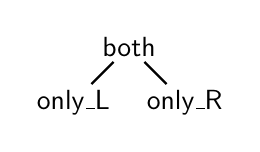
\begin{tikzpicture}
    \node (top) at (0,0) {$\mathsf{both}$};
    \node [below left  of=top] (left)  {$\mathsf{only\_L}$};
    \node [below right of=top] (right) {$\mathsf{only\_R}$};

    % Now draw the lines:
    \draw [thick, shorten <=-2pt, shorten >=-2pt] (top) -- (left);
    \draw [thick, shorten <=-2pt, shorten >=-2pt] (top) -- (right);
\end{tikzpicture}
\end{center}

We can think of opens (in this case $\mathsf{L}$ and $\mathsf{R}$) as behaviors as well, in which case $x \le y$ means that $y$ can always ``choose'' to behave as $x$, in the sense that $y$ could potentially be indistinguishable from $x$. So the Hasse diagram tells us that $\mathsf{both}$ might choose to behave as $\mathsf{only\_L}$ or it may choose to behave as $\mathsf{only\_R}$.

There is a convenient map
\begin{align*}
\mathsf{decide} : \{ (\ell, r) : \Sigma \times \Sigma \suchthat \ell \vee_\Sigma r \} \to \mathsf{Decision}
\\ \mathsf{decide}(\ell, r) = \mathsf{cases}(\ell, r)
\begin{cases}
\fun{(\ell, r)}{\ell}
  \quad &\Longrightarrow \quad \mathsf{only\_L}
\\
\fun{(\ell, r)}{r}
  \quad &\Longrightarrow \quad \mathsf{only\_R}
\end{cases}
\end{align*}
which converts two possible observations $\ell$ and $r$, where we know that one or the other must hold, into a $\mathsf{Decision}$. 

The $\mathsf{cases}$ construct allows one to construct a global definition on a space by providing many local definitions on open subspaces. We can think of it like an overlapping pattern match operation. The syntax of $\mathsf{cases}$, as shown above, suffices to \emph{specify} what the continuous map should do, but we require additional proof to confirm that the local definitions can actually be assimilated into a global definition. These proofs will also determine the computational behavior.

First, the open subspaces of definition must cover the entire space; otherwise, we wouldn't know what to do with the missing parts of the global space! In the example above, this results in the following proof goal
\[
\checkmark(\ell \vee_\Sigma r) \vdash \checkmark(\ell) \vee \checkmark(r),
\]
for $\ell, r : \Sigma$, which is trivial since
\[
\checkmark(\ell \vee_\Sigma r) = \checkmark(\ell) \vee \checkmark(r)
\]
by the definition of $\vee_\Sigma$.

When local definitions overlap, they must be able to be reconciled. That is, suppose we have a point which satisfies several of the possible cases; then, the result should be allowed to behave as if it fell into any of those possible branches. Viewing the specialization order as indicating refinement of possible behaviors, this means that the global result should be the supremum of the results from each of the possible branches.

However, it is not possible in general to take a supremum of points (continuous maps). It's only possible when the supremum is over a set which is \emph{directed} with respect to the specialization order. For instance, in Hausdorff spaces (such as $\R$), where the specialization order is discrete, there are no nontrivial suprema of points. Whenever two branches of a $\mathsf{cases}$ construct overlap, the two local definitions, when restricted to their intersection, must have a maximum.

In the above definition, the overlapping cases can indeed be reconciled. Here, the proof goal is effectively to find a point which is the maximum of $\mathsf{only\_L}$ and $\mathsf{only\_R}$; $\mathsf{both}$ suffices as such a maximum. 

For instance, we have that
\[
\mathsf{decide}(\mathsf{true}, \mathsf{true}) = \dirsup \{ \mathsf{only\_L} , \mathsf{only\_R} \} = \mathsf{both}
\]
since $(\mathsf{true}, \mathsf{true})$ can fall into either branch.


In fact, the two spaces in the type signature of $\mathsf{decide}$ are homeomorphic, with $\mathsf{decide}$ giving one part of that homeomorphism. Its inverse is
\begin{align*}
\mathsf{undecide} &: \mathsf{Decision} \to \{ (\ell, r) : \Sigma \times \Sigma \suchthat \ell \vee_\Sigma r \}
\\ \mathsf{undecide}(d) &= \mathsf{cases}(d)
\begin{cases}
\mathsf{L}
  \quad &\Longrightarrow \quad (\mathsf{true}, \mathsf{false})
\\
\mathsf{R}
  \quad &\Longrightarrow \quad (\mathsf{false}, \mathsf{true})
\end{cases}.
\end{align*}

We can \emph{compute} with $\mathsf{Decision}$s, as with any other space, using open covers. In particular, any $d : \mathsf{Decision}$ decides on either $\mathsf{L}$ or $\mathsf{R}$ by using the \irule{split-cov} rule with the single axiom of the $\mathsf{Decision}$ space, $\top \vdash \mathsf{L} \vee \mathsf{R}$.

So our decision procedure to sound the alarm might look like this:
\begin{align*}
\mathsf{sound\_alarm?} : \R &\to \mathsf{Decision}
\\ \mathsf{sound\_alarm?}(x) &= \mathsf{decide}(x > 4.0, x < 4.1)
\end{align*}

To complete writing this program, we will be presented with a (geometric) proof obligation
\[
x > 4.1 \vee x < 4.0
\]
in the context $x : \R$. What happens when a point satisfies multiple possible cases? Then the decision that is made will depend upon the point's computational behavior. Recall that in the \irule{split-cov} rule, a point much choose an open from an open cover which it lies in. If a point lies in more than 1 of those opens, it may choose any of them, and therefore different implementations of the same point may make different computational choices. So depending on the implementation of a point for the real number 4.05, the alarm may or may not sound.

In comparison with floating point computation, which just branches based on whether $x > 4.0$, computing with $\R$ forces the programmer to explicitly to face the inherent non-determinism inherent in the continuous structure of the real numbers.

So this represents what the naïve computation might look like in formal topology. Now, let's define the inhabited Vietoris powerspace, and accordingly extend the speed estimation example to model worst-case non-determinism.

\subsubsection{Non-determinism with the Vietoris powerspace}

The inhabited Vietoris powerspace $\Viet$ represents non-determinism. For a space $A$, the points of a $\Viet(A)$ are certain ``tractable'' nonempty subspaces of $A$. We will call these subspaces which are points of $\Viet(A)$ \emph{compact/overt}. If a space $A : \Space$ has an open $P : \Open{A}$, then the Vietoris powerspace has opens $\forall x \in \cdot, P(x) : \Open{\Viet(A)}$ as well as $\exists x \in \cdot, P(x) : \Open{\Viet(A)}$. As the notation suggests, viewing $P$ as a proposition that may hold of points of $A$, $\forall x \in \cdot, P(x)$ indicates whether $P$ \emph{necessarily} holds everywhere in the subspace, while $\exists x \in \cdot, P(x)$ indicates whether $P$ \emph{possibly} holds somewhere in the subspace. 

[ Should give more explanation, should say how these are relatively strong computational properties ]

The Heine-Borel theorem states that closed intervals of $\R$ are compact/overt.  It just holds in formal topology: there exists a map
\[
\HeineBorel : \{ (a, b) : \R \times \R \suchthat a < b \} \to \Viet(\R)
\]
such that for every $(a, b) : \R \times \R$ such that $a < b$, we have
\begin{align*}
\forall x \in \HeineBorel(a, b), p < x < q \qquad &\defeq \qquad a < p \wedge q < b
\\ \exists x \in \HeineBorel(a, b), p < x < q \qquad &\defeq \qquad p < b \vee a < q.
\end{align*}

The Heine-Borel theorem has an adjoint: any compact set in $\R$ has a minimum and maximum. So we can define the continuous map $\max : \Viet(\R) \to \R$ as follows:
\begin{align*}
p < \max(s) < q
\qquad \defeq \qquad 
\left( \exists x \in s, p < x \right) \wedge \left( \forall x \in s, x < q \right).
\end{align*}

The Vietoris powerspace is functorial, i.e., applying any continuous map $f : A \to B$ ``pointwise'' to a compact/overt set yields another compact/overt set, so there is a continuous map $\map{\Viet}{f} : \Viet(A) \to \Viet(B)$. The specification of this map is unsurprising:
\begin{align*}
\forall y \in \map{\Viet}{f}(s), P(y) \qquad &\defeq \qquad \forall x \in s, P(f(x))
\\ \exists y \in \map{\Viet}{f}(s), P(y)  \qquad &\defeq \qquad \exists x \in s, P(f(x)).
\end{align*}

Furthermore, the Vietoris powerspace is monadic. For any point $x : A$ there is the compact/overt set $\ret{\Viet}(x) : \Viet(A) $ consisting of that single point:
\begin{align*}
\forall y \in \ret{\Viet}(x), P(y) \qquad &\defeq \qquad P(x)
\\ \exists y \in \ret{\Viet}(x), P(y) \qquad &\defeq \qquad P(x).
\end{align*}
And we can collapse nested nondeterminism in the way we'd expect as well, with $\join{\Viet} : \Viet(\Viet(A)) \to \Viet(A)$:
\begin{align*}
\forall x \in \join{\Viet}(s), P(x) \qquad &\defeq \qquad \forall s' \in s, \forall x \in s', P(x)
\\ \exists x \in \join{\Viet}(s), P(x) \qquad &\defeq \qquad \exists s' \in s, \exists x \in s', P(x).
\end{align*}

Let's use the Vietoris powerspace to enable us to compute with uncertain values of our GPS estimates. Recall that we're imagining that the true position $\ve{x}$ is corrupted by some noise $\ve{n}$ that lies in a closed circular disk, i.e., $\| \ve{n} \| \le \varepsilon$ for some $\varepsilon \ge 0$. For simplicity, assume $\varepsilon = 1$. Then our noise is the unit disk in $\R^2$. We should be able to represent this as a point of $\Viet(\R)$ because it is a compact/overt subspace of $\R^2$. We can explain this in two steps. First, the square 
\[
\{ (x, y) : \R \suchthat -1 \le x \le 1 \wedge -1 \le y \le 1 \}
\]
is compact/overt because it is the product of two intervals, which are each compact/overt by the Heine-Borel theorem. The fact that the product of two compact/overt subspaces is compact is known as the binary Tychonoff theorem, $\otimes : \Viet(A) \times \Viet(B) \to \Viet(A \times B)$. Its specification is given as
\begin{align*}
\forall (a, b) \in s \otimes t, P(a, b)
\qquad &\defeq \qquad
\forall a \in s, \forall b \in t, P(a, b)
\\
\exists (a, b) \in s \otimes t, P(a, b)
\qquad &\defeq \qquad
\exists a \in s, \exists b \in t, P(a, b)
\end{align*}

Next, we know that the unit disk is closed, since it is co-classified by the open set
\[
\fun{(x,y)}{x^2 + y^2 > 1}.
\]
The intersection of a compact/overt space with a closed overt space is still compact/overt\footnote{I need to go back and do this better. I should describe the lower and upper powerspace, so that the closed space being overt is being a point of the upper powerspace}. Given a compact/overt set $s : \Viet{A}$ and an open $U : \Open{A}$ co-classifying a desired closed set, the intersection $s \cap U^c$ is specified by
\begin{align*}
\forall x \in s \cap U^c, P(x) \qquad &\defeq \qquad 
  \forall x \in s, P(x) \vee U(x)
\\
\exists x \in s \cap U^c, P(x) \qquad &\defeq \qquad 
  [[\text{BROKEN}]].
\end{align*}

This yields the desired term $\mathsf{unit\_disk} : \Viet(\R^2)$. Then our speed estimation program which takes into account the uncertainty can be written like this, using ``syntactic sugar'' for monadic operations:
\begin{align*}
\mathsf{compute\_speed}_\Viet : \R^2 \times \R^2 &\to \Viet(\R)
\\ \mathsf{compute\_speed}_\Viet (\ve{x}_1, \ve{x}_2) &= 
  \ve{n}_1 \leftarrow \mathsf{unit\_disk} 
  \then
  \ve{n}_2 \leftarrow \mathsf{unit\_disk}
  \then
  \\ &\ret{\Viet} \left( \mathsf{compute\_speed}(\ve{x}_1 - \varepsilon \ve{n}_1, \ve{x}_2 - \varepsilon \ve{n}_2) \right).
\end{align*}

Note that I subtract the noise rather than add it. Of course, due to symmetries of the unit disk, it doesn't matter here. But there's a small subtlety in the more general case: we imagined that the \emph{real} position was corrupted with some noise which was added to it. But we have the \emph{noisy} position, and want to find all the possible real positions which could yield this noisy one. With any additive noise, we can do this simply via subtraction. However, with a more general noise kernel, this inversion process isn't necessarily so easy.

What do we do now that we have a speed estimate, $s : \Viet(\R)$, which comes with uncertainty, when it comes to deciding whether to sound the alarm. If we use this program
\begin{align*}
\mathsf{sound\_alarm?}_\Viet : \Viet(\R) &\to \mathsf{Decision}
\\ \mathsf{sound\_alarm?}_\Viet(s) &= \mathsf{decide}((\forall x \in s, x > 4.0) , (\exists x \in s, x < 4.1))
\end{align*}
we will be conservative in accordance with our uncertainty; we only sound the alarm if \emph{necessarily} the user's speed is greater than 4mph. Writing this program gives us the proof obligation
\[
\left( \forall x \in s, x > 4.0 \right) \vee \left( \exists x \in s, x < 4.1 \right)
\]
in the context $s : \Viet(\R)$, and intuitively we see that it must hold. Another way to see this is to note the equivalence 
\[
\mathsf{sound\_alarm?}_\Viet(s) = \mathsf{sound\_alarm?}(\max(s)).
\]

The whole program is 
\[
\mathsf{sound\_alarm?}_\Viet \circ \mathsf{compute\_speed}_\Viet : \R^2 \times \R^2 \to \mathsf{Decision}.
\]
Note that the $\Viet$ doesn't occur in the types, as it was only used in intermediate computations. Using $\Viet$ allowed us to conveniently write a program that deals with the uncertainty inherent in GPS coordinates. While it is convenient, it is not necessarily efficient, and in the special case where we have additive noise from the unit disk, we can just do a worst-case speed estimate
\begin{align*}
\mathsf{compute\_max\_speed} &: \{ (\ve{x}_1, \ve{x}_2) : \R^2 \times \R^2 \suchthat \ve{x}_1 \ne \ve{x}_2 \} \to \R
\\ \mathsf{compute\_max\_speed} (\ve{x}_1, \ve{x}_2) &= 
\mathsf{let}\ \ve{d} = \ve{x}_2 - \ve{x}_1\ \mathsf{in}\ 
\\
&\mathsf{compute\_speed}\left( 
\ve{x}_1 - \varepsilon \frac{\ve{d}}{\| \ve{d} \|}, \ve{x}_2 + \varepsilon \frac{\ve{d}}{\| \ve{d} \|}
\right).
\end{align*}
The above program is not defined when $\ve{x}_1 = \ve{x}_2$, butadmits a (unique) continuous extension to the entire space (in this case, the speed estimate when $\ve{x}_1 = \ve{x}_2$ will be $\frac{2\varepsilon}{\Delta t}$)\footnote{I don't know how this construction would actually work in formal topology.}.
Once we've extended the above program, we should be able to prove (with much effort) the equivalence of the programs
\[
\mathsf{sound\_alarm?}_\Viet \circ \mathsf{compute\_speed}_\Viet
=
\mathsf{sound\_alarm?} \circ \mathsf{compute\_max\_speed}.
\]

In this case, we can think of the program which explicitly uses the inhabited Vietoris hyperspace as an executable specification, helping understand when we have found a more efficient program which accomplishes the same task. In particular, the program using $\Viet$ at the very least confirms that it is possible in principle to create such a program.

\subsubsection{How does this beat existing approaches?}

Suppose we simply wanted to program using MLTT, perhaps using data structures for the real numbers from the c-CoRN library. Then one cannot define meaningfully, for instance, the inhabited Vietoris powerspace for $\R$, as notions of continuity and compactness do not interact well, unless one accepts additional axioms. In particular, \cite{waaldijk} proves the following theorem:
\begin{quote}
Within \textsc{bish} the following statements are equivalent:
\begin{enumerate}
\item The fan theorem \textbf{FT}.
\item There exists a class of real-valued functions called `kontinuous' functions such that:
\begin{enumerate}
\item if $f$ is a uniformly continuous real-valued function defined on $[0, 1]$, then $f$ is kontinuous;
\item if $f$ and $g$ are kontinuous functions such that $\text{Ran}(f) \subseteq \text{Dom}(g)$, then the composition $g \circ f$ is kontinuous;
\item if $f$ is a kontinuous function defined on $[0, 1]$, then $f$ is
uniformly continuous;
\item the function $x \mapsto 1/x$, defined on $\R^+$, is kontinuous.
\end{enumerate}
\end{enumerate}
\end{quote}

Therefore, even \emph{reasoning} about such ideas is difficult in MLTT, and certainly there is no in-built mechanism for \emph{computing} in this manner. Whilst there may be ways around these difficulties, at the very least the concepts are not natural. So in MLTT, the best one could do is reason about nondeterminism using definitions as subsets of points; computing over those subsets is not possible.

Most of the concepts described thus far are also described in a similar way in Paul Taylor's Abstract Stone Duality (ASD). However, as far as I am aware, there is no notion of the $\mathsf{cases}$ construct in ASD, which is needed to make discrete decisions over connected spaces. The Marshall programming language is capable of doing some of the interesting computation described here, such as universal quantification over the unit disk\footnote{I'm still unsure about existential quantification over the unit disk, in general.}. However, since its only base type is $\R$, it does not have, for instance, the Vietoris powerspace as a first-class object.

[[Compare to dReal]]

[What other alternative approaches are there that I should claim are not as good as this approach?]

\subsubsection{The probabilistic powerspace}

Likewise, we can form a topological space for all probability distributions over a given space. Let's describe the space $\Prob(A)$ of probability distributions over some space $A$. Let $\ratint = \{q : \rat \suchthat 0 \le q < 1 \}$. For each $P : \Open{A}$ and each $q : \ratint$, the basic open $\cdot(P) > q : \Open{\Prob(A)}$ which indicates whether the probability that the event $P$ occurs is strictly greater than $q$.

We can generalize a bit further: given any topological space $A$, we can form a topological space of its open subspaces $\mathsf{Open}(A)$, whose points consist of open subspaces of $A$, and whose topology is the Scott topology. We can also define a topological space $\lowerT{\R}$ known as the \emph{lower real numbers}, where the basic opens are of the form $\cdot > q : \Open{\lowerT{\R}}$ for $q : \rat$. Interestingly, both $\mathsf{Open}(A)$ and $\lowerT{\R}$ are Scott domains, which means that any open cover has singleton subcover [[This seems wrong. What about covers which come from ``below''?]]. Thus, being a Scott domain is a sort of ``ultra''-compactness. The probability space $\Prob(A)$ can be seen as a subspace of the function space $\mathsf{Open}(A) \Rightarrow \lowerT{\R}$. \footnote{The function space $X \Rightarrow Y$ does not necessarily exist (in the sense of being the categorical exponential) for arbitrary spaces $X$ and $Y$, but does exist whenever $X$ is a Scott domain (a sufficient but not necessary condition), as it is in this case, where $X = \mathsf{Open}(A)$.}

In particular, viewing $\Prob(A)$ as a subspace of $\mathsf{Open}(A) \Rightarrow \lowerT{\R}$, we additionally require the following rules to hold for any $\mu : \Prob(A)$
\begin{mathpar}
\mu(\bot_A) = 0
\\ \mu(\top_A) = 1
\\ \frac{P \to Q}{\mu(P) \le \mu(Q)}
\\ \mu(P \vee Q) + \mu(P \wedge Q) = \mu(P) + \mu(Q).
\end{mathpar}

It is not at all obvious that these laws can be presented as geometric theories. \cite{vickers2011} gives a geometric presentation.

Perhaps more important than understanding the exact formal phrasing of the axioms is getting a feeling for what kinds of observations one can make on $\Prob(A)$. In particular, we can investigate what open covers one may form on $\Prob(A)$. Given an open cover $\top \vdash \bigvee_{i : I} P_i$ of $A$, and given rational numbers $q_i : \ratint$ for each $i : I$ such that $\sum_{i : I} q_i < 1$, we have the open cover
\[
\top \vdash \bigvee_{i : I} \cdot(P_i) > q_i
\]
on $\Prob(A)$. Not every open cover looks like this, but this is a particularly useful form, particularly in the context of decision making.

Like the Vietoris powerspace, the probabilistic powerspace is also functorial, meaning that we can apply a continuous map $f : A \to B$ to a probability distribution $\Prob(A)$ to get a probability distribution $\Prob(B)$ (with the expected properties), which can be specified as
\[
\map{\Prob}{f}(\mu)(P) > q \qquad \defeq \qquad \mu(f^{-1}P) > q.
\]

The probabilistic powerspace is also monadic. For a point $x : A$ there is the probability distribution which has all its mass at that single point,
\[
\ret{\Prob}(x)(P) > q \qquad \defeq \qquad P(x).
\]

And we can collapse nested probability distributions via integration in the way we'd expect as well, with $\join{\Prob} : \Prob(\Prob(A)) \to \Prob(A)$:
\[
\join{\Prob}(\mu)(P) > q \qquad \defeq \qquad
   \int_{\nu \in \Prob(A)} \nu(P) d\mu(\nu) > q.
\]

It's not obvious that the right-hand side of the above definition is in fact an open set; what we're claiming is that the integral results in a lower real number. In fact, integration gives a continuous map $\int : (X \Rightarrow \lowerT{\R}) \times \Prob(X) \to \lowerT{\R}$ \cite{vickersintegral} (whenever the function space $X \Rightarrow \lowerT{\R}$ exists, which is whenever $X$ is locally compact; here we have $X = \mathsf{Prob}(A)$ which is apparently locally compact).

The $\map{\Prob}$ function also allows us to define the tensorial strength for $\Prob$, $\mathsf{strength}_\Prob : A \times \Prob(B) \to \Prob(A \times B)$ by
\[
\mathsf{strength}_\Prob(x, \mu)
\qquad \defeq \qquad
\map{\Prob}(\fun{y}{(x, y)})(\mu).
\]
\cite{vickers2011} shows that indeed $\Prob$ forms a commutative monad.

We should be able to form the normal distribution, $\mathcal{N} : \R \times \{ \sigma^2 : \R \suchthat \sigma^2 \ge 0 \} \to \Prob(\R)$. The construction is likely involved and beyond the scope of this article.

With these definitions in place, we can use the probabilistic powerspace to compute with probabilistically uncertain GPS estimates. Recall that we're imagining that the true position $\ve{x}$ is corrupted by some noise $\ve{n}$ drawn from a normal distribution $\mathcal{N}(0, \sigma^2)$ with mean $0$ and variance $\sigma^2$. We can now compute the probability distribution which represents what speed we believe the walker has, by defining
\begin{align*}
\mathsf{compute\_speed}_\Prob : \R^2 \times \R^2 &\to \Prob(\R)
\\ \mathsf{compute\_speed}_\Prob (\ve{x}_1, \ve{x}_2) &= 
  \ve{n}_1 \leftarrow \mathsf{noise}(\sigma^2)
  \then
  \ve{n}_2 \leftarrow \mathsf{noise}(\sigma^2)
  \then
  \\ &\ret{\Prob} \left( \mathsf{compute\_speed}(\ve{x}_1 - \ve{n}_1, \ve{x}_2 - \ve{n}_2) \right),
\end{align*}
where
\begin{align*}
\mathsf{noise} &: \{ \sigma^2 : \R \suchthat \sigma^2 \ge 0 \} \to \Prob \left( \R^2 \right)
\\ \mathsf{noise}(\sigma^2) &= 
  x \leftarrow \mathcal{N}(0, \sigma^2)
  \then
  y \leftarrow \mathcal{N}(0, \sigma^2)
  \then
  \ret{\Prob}(x, y).
\end{align*}

Note the similarity between this function and $\mathsf{compute\_speed}_\Viet$. We may then wish to decide whether or not to sound the alarm using the procedure
\begin{align*}
\mathsf{sound\_alarm?}_\Prob : \Prob(\R) &\to \mathsf{Decision}
\\ \mathsf{sound\_alarm?}_\Prob(\mu) &= 
  \mathsf{decide}(\mu(\cdot > 4.0) > 0.9 , \mu(\cdot < 4.1) > 0.05),
\end{align*}
which again is fairly conservative: we will only sound the alarm if we're more than 90\% sure that the user's speed is greater than 4mph.

The whole program using the probabilistic approach,
\[
\mathsf{sound\_alarm?}_\Prob \circ \mathsf{compute\_speed}_\Prob : \R^2 \times \R^2 \to \mathsf{Decision},
\]
requires computing a double integral over two normal distributions, which is not necessarily efficient. We can reduce the computational burden by making a few observations. First, for any $\ve{x}_1, \ve{x}_2, \ve{n}_1, \ve{n}_2 : \R^2 $ we have
\[
\mathsf{compute\_speed}(\ve{x}_1 - \ve{n}_1, \ve{x}_2 - \ve{n}_2)
= 
\mathsf{compute\_speed}(\ve{x}_1  + (\ve{n}_2 - \ve{n}_1), \ve{x}_2),
\]
and secondly, we should be able to prove that
\[
  \ve{n}_1 \leftarrow \mathsf{noise}(\sigma^2)
  \then
  \ve{n}_2 \leftarrow \mathsf{noise}(\sigma^2)
  \then
  \\ \ret{\Prob}(\ve{n}_1 - \ve{n}_2)
= \mathsf{noise}(2\sigma^2).
\]

With these facts, we can compute the speed estimate in the following more efficient manner,
\begin{align*}
\mathsf{compute\_speed'}_\Prob : \R^2 \times \R^2 &\to \Prob(\R)
\\ \mathsf{compute\_speed'}_\Prob (\ve{x}_1, \ve{x}_2) &= 
  \ve{n} \leftarrow \mathsf{noise}(2 \sigma^2)
  \then
  \ret{\Prob} \left( \mathsf{compute\_speed}(\ve{x}_1 - \ve{n}, \ve{x}_2) \right).
\end{align*}

With some more careful statistics, it may be possible to write an even more efficient computation of the decision procedure that doesn't even involve any use of probability distributions.

\section{Car approaching a traffic light}

Suppose we have a car which is approaching a traffic light which has just turned yellow. Should it stop for the light, or should it go through the intersection?

Concretely, let's imagine that the only variable affecting the car's decision should be its position $y : \R$ at the time the light turns yellow. Let $0 : \R$ indicate the position of the intersection. We require that the car's position $r : \R$ when the light turns red satisfies
\[
y + 1< r < y + 2 \quad \wedge \quad r \ne 0,
\]
meaning that the car not be exactly at the intersection when the light turns red, and that it must move between 1 and 2 units forward between the yellow and red light. The proposition $r < 0$ indicates choosing to stop, while $r >0$ indicates choosing to go.

Thus, it's safe to stop as long as $y < -1$ and safe to go as long as $y > -2$. So our decision-making procedure is:
\begin{align*}
\mathsf{stop?} &: \R \to \PLower(\bool)
\\ \mathsf{stop?}(y) &= \mathsf{cases}(y)
\begin{cases}
\cdot < -1
  \quad &\Longrightarrow
   \ret{\PLower} (\mathsf{true})
\\
\cdot > -2
  \quad &\Longrightarrow
   \ret{\PLower}(\mathsf{false}).
\end{cases}
\end{align*}

Since any two (generalized) points of the powerspace $\PLower(A)$ for any space $A$ have a maximum (defined as the union of overt subspaces), we must only check that the cases given indeed cover the full space,
\[
\top_\R \quad \vdash \quad \cdot < -1 \quad \vee \quad \cdot > -2.
\]

However, likely the estimate of the car's position is noisy. If we model with non-deterministic noise, then a first attempt at the stopping decision procedure might be
\begin{align*}
\mathsf{stop?} &: \Viet(\R) \to \PLower(\bool)
\\ \mathsf{stop?}(s) &= \mathsf{cases}(s)
\begin{cases}
\forall x \in \cdot, x < -1
  \quad &\Longrightarrow
   \ret{\PLower} (\mathsf{true})
\\
\forall x \in \cdot, x > -2
  \quad &\Longrightarrow
   \ret{\PLower}(\mathsf{false}).
\end{cases}
\end{align*}

The argument $s : \Viet(\R)$ to $\mathsf{stop?}$ indicates the (compact/overt) subspace of possible positions of the car. The opens given in the $\mathsf{cases}$ construct use universal quantification to ensure that a decision is made only when it is \emph{necessarily} safe for \emph{any} possible position of the car.

However, it is impossible to satisfy the proof obligation for the above definition, because the cases do not cover the entire space $\Viet(\R)$. For instance, the closed interval $[-3, 0]$ considered as a point of $\Viet(\R)$ satisfies neither of the two propositions.\footnote{It is not always the case that a logical statement which is not provable has a counterexample; for instance, there are nontrivial locales with no (global) points at all.}

A trivial solution is to restrict the input to be exactly which is in the open subspace that is covered, i.e., modify the type signature to
\[
\mathsf{stop?} : \{ s : \Viet(\R) \suchthat 
 \left(\forall x \in s, x < -1 \right) \vee \left(\forall x \in s, x > -2 \right)
 \} \to \PLower(\bool).
\]

But perhaps more interesting is to imagine that perhaps the uncertain noise takes a particular form, such as a closed ball of a fixed radius $\delta : \R$ about a center point,
\begin{align*}
\mathsf{stop?} &: \R \to \PLower(\bool)
\\ \mathsf{stop?}(c) &= \mathsf{cases}(\HeineBorel(c - \delta, c + \delta))
\begin{cases}
\forall x \in \cdot, x < -1
  \quad &\Longrightarrow
   \ret{\PLower} (\mathsf{true})
\\
\forall x \in \cdot, x > -2
  \quad &\Longrightarrow
   \ret{\PLower}(\mathsf{false}).
\end{cases}
\end{align*}
This first yields the proof goal
\[
\top \vdash \cdot - \delta < \cdot + \delta
\]
which ensures that the closed interval $[c - \delta, c + \delta]$ is inhabited, and also gives the proof goal in the context $c : \R$
\[
\left( \forall x \in \HeineBorel(c - \delta, c + \delta), x < -1 \right)
\quad \vee \quad
\left( \forall x \in \HeineBorel(c - \delta, c + \delta), x > -2 \right)
\]
which reduces to
\[
c + \delta < -1  \quad \vee \quad
c - \delta > - 2
\]
which can be proved as long as $0 < \delta < 1$.

In fact, we need to decide not only whether to stop or go, but also how far the car should move forward between the yellow and red light (which, by our toy laws of physics, must be strictly between 1 and 2 units of distance).\footnote{If we didn't make the ranges narrower, we'd need to make the choice depend on the distance, which is possible, but slightly more complicated. Even when taking into account whether to stop or go, this amount must depend on the car's distance: if a car's position is $-(1 + \varepsilon)$ for some small $\varepsilon > 0$, then it must move forward by some distance $d : \R$ such that $1 < d < 1 + \varepsilon$.} 
The following program satisfactorily determines how far to move forward
\begin{align*}
\mathsf{forward} &: \R \to \PLower(\{ d : \R \suchthat 1 < d < 2 \})
\\ \mathsf{forward}(c) &= \mathsf{cases}(\HeineBorel(c - \delta, c + \delta))
\begin{cases}
\forall x \in \cdot, x < -1.1
  \quad &\Longrightarrow
   \ret{\PLower}(1.1)
\\
\forall x \in \cdot, x > -1.9
  \quad &\Longrightarrow
   \ret{\PLower}(1.9),
\end{cases}
\end{align*}
and is a valid definition as long as $\delta < 0.8$.

[ The following is wrong. I didn't make it the lower powerspace for the distance to move forward. But then the condition is no longer an open subspace, which is annoying.]
Finally, we may wish to write a program whose type signature captures entirely the requirement that the car's position when the light turns red. The dependent type signature
\begin{align*}
\mathsf{stoplight} &: \forall s : \{ s' : \Viet(\R) \suchthat U(s') \},
  \exists d : \{ d' : \R \suchthat 1 < d' < 2 \},
  \forall x \in s,  x + d \ne 0
\end{align*}
captures all of these aspects (where $U$ ought to be some predicate which makes the above type inhabitable). Note that the first $\forall$ and $\exists$ symbols in the above type are different than the notation used for points of the powerspaces; the usage of the colon rather than $\in$ is meant to signify this difference.

The meaning of the above type is that one must actually produce the simply typed continuous map
\begin{align*}
\mathsf{stoplight}' &: \{ s' : \Viet(\R) \suchthat U(s') \}
  \to \{ (s, d) : \{ s' : \Viet(\R) \suchthat U(s') \} \times \{ d' : \R \suchthat 1 < d' < 2 \}
                   \suchthat \forall x \in s, x + d \ne 0 \}
\end{align*}
with the additional requirement that
\[
\mathsf{fst} \circ \mathsf{stoplight}' = \mathsf{id}.
\]
This translation is just the categorical interpretation of dependent types as overcategories (also known as slice categories).

\section{Differential equations and thermostats}

\cite{smooth-interp} presents an example where a thermostat controls the temperature of a room by periodically reading the temperature of the room and switching a heater on and off.  Differential equations specify the dynamics of the room's temperature. We will model this example with formal topology.

\subsubsection{Solving differential equations}

The Picard-Lindelöf theorem is probably the simplest theorem which allows for the solution of differential equations. The Picard-Lindelöf construction would consist of several steps.

A key component of Picard-Lindelöf is the contraction mapping principle, a theorem concerning metric spaces. I have completed the ``localic metric completion'' construction, which produces as a topological space the metric completion of a \emph{set} of points $X$ together with a metric $\delta_X : X \times X \to \upperT{\R}$, where $\upperT{\R}$ is the space of non-negative real numbers (including $\infty$) with the upper topology. The metric $\delta_X$ is extended to a continuous map $\delta : \mathfrak{C}(X) \times \mathfrak{C}(X) \to \upperT{\R}$, where $\mathfrak{C}(X)$ is the metric completion of $X$.
For instance, the space of metric real numbers $\R$ are defined as the completion of the set of rational numbers $\rat$.

An additional construction I would need to add is that any Cauchy net\footnote{A net is a generalization of a sequence from the directed set of natural numbers (with the standard order) to arbitrary directed sets.} has a limit point. This would be phrased as a construction on \emph{generalized} points of the metric space $X$, i.e., continuous maps $\Gamma \to X$ for an arbitrary space $\Gamma$.

For a metric space $X$ with metric $\delta$, a map $T : X \to X$ is defined as a \emph{contraction mapping} if there is some $q : \rat$ such that one can prove for arbitrary $x, y : X$ and every $r : \rat$ the geometric implication
\[
\delta(x, y) < r
\quad \vdash \quad
\delta(T(x), T(y)) < q r,
\]
which in more familiar (classical) language says that $\delta(T(x), T(y)) \le q \delta(x, y)$.\footnote{I might have a difficulty dealing with the fact that $\infty$ is allowed in $\upperT{\R}$.}

The contraction mapping principle says that a contraction mapping $T : X \to X$ has a fixed point $x^*$ such that $T(x) = x$ (assuming $X$ is inhabited). This follows from the fact that, given any point $x_0 : X$, the sequence $x_n \defeq T^n(x_0)$ is Cauchy; in fact, it converges at a geometric rate, as
\[
\delta(x^*, x_n) \le \frac{q^n}{1 - q} \delta(x_1, x_0).
\]

The Picard-Lindelöf theorem states that for any Lipschitz function $f : \R^n \times R$, there is a continuous map $\mathsf{PL}_f : \R^n \times \R \times \R \to \R^n$ such that for any $t_i, t_f : \R$ and $x_0 : \R^n$, $\mathsf{PL}_f(x_0, t_i, t_f)$ is the unique solution $x(t_f)$ of the differential equation specified by
\begin{align*}
\frac{dx}{dt} &= f(x, t)
&
x(t_i) &= x_0.
\end{align*}
Its constructive nature, in using the contraction mapping principle, means that Picard-Lindelöf too is constructive.

\subsubsection{Simulating temperature change}

The temperature change in the room is modeled by Newton's law of cooling. Let $\mathsf{on} : \bool$ indicate whether the heater is currently on, and define $\mathsf{heat} : \bool \to \R$ by
\begin{align*}
\mathsf{heat}(\mathsf{true}) &= h
&
\mathsf{heat}(\mathsf{false}) &= 0
\end{align*}
for some constant $h : \R$. Then the temperature's dynamics are governed by the equation
\[
\frac{dT}{dt} = -kT + \mathsf{heat}(\mathsf{on}),
\]
that is, the dynamics are governed by the functions
\begin{align*}
f_\mathsf{true}(T, t) &= -kT + h
\\ f_\mathsf{false}(T, t) &= -kT,
\end{align*}
where $T$ indicates the temperature (in Kelvin) and $k : \R$ is some positive constant. Clearly this equation is Lipschitz with Lipschitz constant $k$, so we can simulate the temperature's change using the Picard-Lindelöf construction.

Concretely, the temperature's dynamics are given by
\begin{align*}
\mathsf{temp} &: \bool \times \R \times R \to \R
\\ \mathsf{temp}(\mathsf{true}, T_i, t) &= \mathsf{PL}_{f_\mathsf{true}}(T_i, 0, t)
\\ \mathsf{temp}(\mathsf{false}, T_i, t) &= \mathsf{PL}_{f_\mathsf{false}}(T_i, 0, t),
\end{align*}
where the arguments to $\mathsf{temp}$ are the whether the heater is on, the initial temperature $T_i$, and the time $t$ to check the temperature.

Furthermore, we should be able to prove that the solution to this differential equation is
\[
T(t_f) = \left( T(t_i) - \frac{\mathsf{heat}(\mathsf{on})}{k}\right) \exp\left(-kT(t_f - t_i) \right) + \frac{\mathsf{heat}(\mathsf{on})}{k}.
\]
Using the above definition may be more efficient than the definition using Picard-Lindelöf. It might depend on the definition of $\exp$, for which one of the canonical definitions is as the solution of an ODE.

\subsubsection{Controlling the thermostat}

Periodically, the thermostat decides to switch itself on or off. We imagine that the thermostat reads some temperature $T : \R$ as its input and additionally has access to the variable $\mathsf{on} : \bool$ which indicates whether the heater is currently on. We might imagine that the temperature sensor is not perfect, and use a probabilistic model $\mu : \R \to \Prob(\R)$ which produces a probability distribution expressing our belief in the current temperature given the sensor reading. One way to control the thermostat would be with this definition:
\begin{align*}
\mathsf{control} &: \R \times \bool \to \PLower(\bool)
\\
\mathsf{control}(T, \mathsf{true}) &= 
\mathsf{cases}(\mu(T))
\begin{cases}
\cdot(\cdot > T_\text{off}) > 0.9
  \quad &\Longrightarrow
  \ret{\PLower}(\mathsf{false})
\\
\cdot(\cdot < T_\text{off} - \varepsilon) > 0.1
  \quad &\Longrightarrow
  \ret{\PLower}(\mathsf{true})
\end{cases}
\\
\mathsf{control}(T, \mathsf{false}) &= 
\mathsf{cases}(\mu(T))
\begin{cases}
\cdot(\cdot < T_\text{on}) > 0.9
  \quad &\Longrightarrow
  \ret{\PLower}(\mathsf{true})
\\
\cdot(\cdot > T_\text{on} + \varepsilon) > 0.1
  \quad &\Longrightarrow
  \ret{\PLower}(\mathsf{false}),
\end{cases}
\end{align*}
where $T_\text{off}$ is the temperature above which we'd like to turn the heater off if it is already on, $T_\text{on}$ is the temperature below which we'd like to turn the heater on if it is currently off, and $\varepsilon > 0$ is a constant indicating the precision (in terms of temperature) with which we'd like to make the decision. It makes sense to set $T_\text{on} <  T_\text{off}$ to avoid switching the heater on and off too frequently.

This decision procedure is relatively ``conservative'' in deciding to switch the heater on or off, in that it must be at least 90\% confident that the threshold has been exceeded. Imagine if the temperature sensor were very inaccurate, such that the distribution $\mu(T)$ is very broad. If we only required a low degree of confidence, say 10\%, then it may be the case the thermostat would unnecessarily turn the heater on and off too frequently due to its inaccurate assessment of the current temperature. The above control procedure avoids such an issue.

Let's put the whole simulation together. We'll assume that the thermostat's control routine $\mathsf{control}$ is called once per unit of time.

\begin{align*}
\mathsf{sim} :\ & \nat \times \bool \times \R \times \R \to \PLower(\Prob(\R \times \bool))
\\
\mathsf{sim}(0, \mathsf{on\_init}, T_i, t) = 
  &\ret{\PLower \circ \Prob}(\mathsf{temp}(\mathsf{on\_init}, T_i, t), \mathsf{on\_init})
\\
\mathsf{sim}(S(n), \mathsf{on\_init}, T_i, t) = 
&(T, \mathsf{on}) \leftarrow \mathsf{sim}(n, \mathsf{on\_init}, T_i, 1)
 \then
 \\&T_\text{meas} \leftarrow \ret{\PLower}(\nu(T))
 \then
 \\ &\mathsf{on}' \leftarrow \map{\PLower}(\ret{\Prob})(\mathsf{control}(T_\text{meas}, \mathsf{on}))
 \then
 \\ &T_f \leftarrow \mathsf{temp}(\mathsf{on'}, T, t)
 \then
 \\ &\ret{\PLower \circ \Prob}(T_f, \mathsf{on'}).
\end{align*}

The probability distribution $\nu : \R \to \Prob(\R)$ gives the probability distribution of the temperature that the thermostat measures as a function of the actual temperature.

The arguments to $\mathsf{sim}$ are as follows: the first and last arguments are supposed to represent the amount of time since the simulation started, where the first argument $n$ is the number of whole minutes which have elapsed, and the final argument $t$ is the additional fraction of a minute which has elapsed, i.e., we require $0 \le t \le 1$, and imagine that the total time elapsed is $n + t : \R$. Note that, given an arbitrary real number, it is not possible to decompose it into an integral and fractional part, hence, we require them as separate arguments. The middle two arguments, $\mathsf{on\_init}$ and $T_i$, are the state of the heater and the temperature of the room at the very beginning of the simulation.

Even though $\mathsf{sim}$ requires that the simulated time be decomposed into an integral and fractional part, this should not be necessary, since in fact the temperature of the room varies continuously with time, even at the moment when the heater switches on or off. It would be possible to stitch together all of the pieces together to get a single simulator function which simply takes a time argument as a real number by proving that the pieces agree on their endpoints,\footnote{I haven't actually thought through the details of how this construction would work. There's a simple way to stick together two pieces, but infinitely many is a bit more complicated.} i.e.,
\[
\mathsf{sim}(n, \mathsf{on\_init}, T_i, 1) = \mathsf{sim}(S(n), \mathsf{on\_init}, T_i, 0).
\]

A final interesting thing to note with the $\mathsf{sim}$ function is the composition of non-determinism and probability monads. [I need to explain why these two monads compose. I believe that consists of giving a commutator.] Note that these monads do not commute with each other. Probability arises because of the probabilistic nature of the thermostat's sensor reading, while non-determinism arises because the thermostat must make a discrete decision over a connected space.

\subsubsection{Running the simulations}

I have yet to discuss in detail how ``run'' continuous maps. First, notice that it only really makes sense to run points of a space, rather than arbitrary continuous maps. That is, a continuous map should first be applied to concrete values of arguments to produce an output value which is just a point of the output space.

The key to ``running'' points is to pick an informative open cover that discriminates the properties you wish to observe, and then use the \irule{split-cov} rule to determine which open holds of the particular point that is being observed. For instance, we can cover $\R$ with open balls of radius $\varepsilon : \rat^+$ centered at every possible rational number. Using the \irule{split-cov} rule with this cover, we can approximate a point $x : \R$ by finding some rational number $q : \rat$ such that $|q - x| < \varepsilon$. Note that there is inherent non-determinism here, in that different representations of the same real number may yield different rational approximations.

We can define a simple type 
\begin{align*}
\mathsf{Approx} &: \Space \to \Type \to \Type
\\ \mathsf{Approx}\ A\  I &= \left\{ P : I \to \Type \suchthat \top \vdash \bigvee_{i : I} P_i \right\}
\end{align*}
which is the type of approximations of a given space. For instance, as explained above, there is a function $\mathsf{rat\_approx} : \rat^+ \to \mathsf{Approx}\ \R\ \rat$ which gives rational approximations of real numbers.

There is a simple and natural way to approximate product spaces. Suppose we have two spaces $A$ and $B$. Given an open cover $\bigvee_{i : I} P_i$ of $A$ and an open cover $\bigvee_{j : J} Q_j$ of $B$, we can produce the cover $\bigvee_{(i, j) : I \times J} P_i \times Q_j$ of $A \times B$. Accordingly, given approximators $\mathsf{approx}_A : \mathsf{Approx}\ A\ I$ and $\mathsf{approx}_B : \mathsf{Approx}\ B\ J$, there is the product approximator
\[
\mathsf{approx}_A \times \mathsf{approx}_B : \mathsf{Approx}\ (A \times B)\ (I \times J).
\]

Approximating discrete spaces is easy. If $\mathsf{Disc} : \Type \to \Space$ constructs a discrete space from its underlying set, then $\mathsf{approx\_Disc} : \forall A : \Type, \mathsf{Approx}\ (\mathsf{Disc}\ A)\ A$ converts a point of the space $\mathsf{Disc}\ A$ back into an element of $A$.

It is straightforward to simulate a non-deterministic run of the non-determinstic powerspaces $\PLower$ as well as $\Viet$ (given that $\Viet$ is a subspace of $\PLower$). If we have a space $A$ with an open cover $\bigvee_{i : I} P_i$, then there is the cover
\[
\bigvee_{i : I} \exists x \in \cdot, P_i(x)
\]
of $\PLower(A)$. So given $a : \mathsf{Approx}\ A\ I$, we have the approximator $\mathsf{possible}(a) : \mathsf{Approx}\ (\PLower(A))\ I$ which returns a \emph{possible} run of the non-determinism.

Simulating probabilistic non-determinism is more complicated. Suppose we have a space $A$ and an open cover $\bigvee_{i : I} P(i)$. What can we do with it?

We might like to compute the probability of each $P(i)$. However, this cannot be done in general. For instance, consider probability distributions over the Sierpínski space $\Sigma$. The probability of landing in the non-trivial open is just a non-negative lower real number, and since the non-negative lower reals have a bottom element (0), it is very weak computationally.

A more realistic ambition is to realize that there must be a way to distribute weight into each open $P_i$ in a consistent manner. That is, we should be able to break the number 1 into a sum $1 = \sum_{i : I} x_i$ of non-negative real numbers $x : I \to \R$ such that each $x_i$ is no greater than the probability of $P_i$. If each of the $P_i$ happen to be clopen, and hence the $P_i$ are pairwise disjoint, then there is only one such decomposition, and indeed each corresponding $x_i$ represents the probability of each $P_i$. However, if there is overlap among the open cover, there is choice in how to distribute the weight which lies in the intersection, and there is no reason to expect that this distribution can be done canonically, that is, different representations of the same probability distribution might result in different decompositions.

Here is a rough sketch of how this decomposition works. Suppose we have $\mu : \Prob(A)$. We have $\mu(\top) = 1$, but by monotonicity, since
\[
\top \dashv \vdash \bigvee_{i : I} P_i
\]
then $\mu\left( \bigvee_{i : I} P_i \right) = 1$ as well. By continuity, it suffices to consider the supremum of finite joins, so
\[
\sup_{\ell : \mathcal{FP}(I)} \mu \left( \bigvee_{x \in \ell} P_x \right) = 1,
\]
where $\mathcal{FP}(I)$ denotes the type of lists of elements of $I$, i.e., the Kuratowski-finite powerset of $I$. This means that for all $q : \rat$ such that $q < 1$, there exists some $\ell : \mathcal{FP}(I)$ such that
\[
\mu \left( \bigvee_{i \in \ell} P_i \right) > q.
\]

If the list $\ell$ is nonempty, that is, $\ell = i :: is$ for some $i : I$ and $is : \mathcal{FP}(I)$, then by modularity we have
\[
\mu(P_i) +  \mu \left( \bigvee_{j \in is} P_j \right) = 
 \mu \left( P_i \vee \bigvee_{j \in is} P_j \right) + \mu \left( P_i \wedge \bigvee_{j \in is} P_j \right),
\]
hence, combining the above two equations,
\[
\mu(P_i) +  \mu \left( \bigvee_{j \in is} P_j \right) > q,
\]
and therefore there exist $q_i, q_{is} : \rat$ such that $q_i + q_{is} = q$ and
\begin{align*}
\mu(P_i) > q_i \quad \text{and} \quad  \mu \left( \bigvee_{j \in is} P_j \right) > q_{is}.
\end{align*}

Recursively repeating this process yields rational numbers $q_i : \rat$ for each $i : I$ such that $\mu(P_i) > q_i$ and also $\sum_{i : I} q_i > q$, and this can be done for any $q < 1$. Hence, for every $q < 1$, there is the open cover
\[
\top \vdash \bigvee_{\ell : \mathcal{FP}(I \times \rat)} \left(
\sum_{(i, q_i) \in \ell} q_i = q \quad \wedge \quad \forall \ell' \subseteq \ell, \mu\left( \bigvee_{(i, q_i) \in \ell'} P_i \right) > \sum_{(i, q_i) \in \ell'} q_i \right)
\]
(the universal quantification is okay since there are finitely many sublists of a finite list, so it is just a finitary conjunction).

Therefore, for a space $A$ with approximator $a : \mathsf{Approx}\ A\ I$, we have the approximator $\mathsf{prob}(a) : \{ q : \rat \suchthat q < 1 \} \to \mathsf{Approx}\ (\Prob(A))\ (\mathcal{FP}(I \times \rat))$ which returns an approximation to a distribution of the weight of probability amongst the open cover. Though I will not go into the explanation, this should allow one to recover a function $\mathsf{Pt}(A) \to (I \to \R)$ which non-deterministically assigns a real-valued number weight to each open such that the total weight assigned is exactly 1.

We can compose these approximators together to simulate the thermostat. We can compose the approximator
\begin{align*}
\mathsf{run\_sim} : \rat \times \rat &\to \mathsf{Approx}\ (\PLower(\Prob(\R \times \bool)))\ (\mathcal{FP}((\rat \times \bool) \times \rat))
\\
\mathsf{run\_sim}(\varepsilon, q) &= 
\mathsf{possible}(\mathsf{prob}(\mathsf{rat\_approx}(\varepsilon) \times \mathsf{approx\_Disc})(q)).
\end{align*}

This approximator takes two arguments, $\varepsilon$ and $q$, which represent tolerance/approximation parameters. The basic open sets of the underlying space $\R \times \bool$ look like open balls of radius $\varepsilon$ about rational centers, which approximate the temperature, together with boolean values which indicate whether the heater is on. The approximator returns a list of these basic opens, together with weights which lower bound the probability of that open as well as its union with other opens in the list, and for which the total weight is $q$.

\subsubsection{Optimizing thermostat behavior}

We may wish to set the parameter $T_\text{on}$ and $T_\text{off}$ such that the room's temperature is close to the desired temperature. We'll begin by simplifying the thermostat scenario from the model that was posed above. Imagine that there is a function $\mathsf{sim} : \R \times \R \times \R \to \R$, where $\mathsf{sim}(T_\text{on}, T_\text{off}, t)$ returns the temperature of the room at time $t$ if the thermostat is operated with temperature thresholds $T_\text{on}$ and $T_\text{off}$.

Suppose that we have an optimal temperature trajectory $\tau : [0, t_f] \to \R$ which gives the desired temperature as a function of time, up until the end time, $t_f$. We then may wish to choose $T_\text{on}$ and $T_\text{off}$ to minimize the quantity
\[
\mathsf{error}(T_\text{on}, T_\text{off}) \defeq \int_0^{t_f} (\mathsf{sim}(T_\text{on}, T_\text{off}, t) - \tau(t))^2 dt.
\]
\cite{vickersintegral} explains how the Riemann integral can be defined such that the above quantity is simply computable. Moreover, suppose we know we will restrict our choices of $T_\text{on}$ and $T_\text{off}$ to the compact/overt sets $\mathsf{on}, \mathsf{off} : \Viet(\R)$. Then we can just compute the minimum error,
\[
\mathsf{min\_error} \defeq \min(\map{\Viet}\mathsf{error}(\mathsf{on} \otimes \mathsf{off})).
\]
Then, note that for any $\varepsilon > 0$, we can derive
\[
\top \quad \vdash \quad \mathsf{min\_error} < \mathsf{min\_error} + \varepsilon,
\]
which by reduction gives
\begin{align*}
\top \quad \vdash \quad &\min(\map{\Viet}\mathsf{error}(\mathsf{on} \otimes \mathsf{off})) < \mathsf{min\_error} + \varepsilon
\\ \top \quad \vdash \quad &\exists (T_\text{on}, T_\text{off}) \in (\mathsf{on} \otimes \mathsf{off}), \mathsf{error}(T_\text{on}, T_\text{off}) < \mathsf{min\_error} + \varepsilon.
\end{align*}
By the rules of non-deterministic powerspaces, for any space $A$, open $U$ of $A$, and open cover $\bigvee_{i : I} P_i$ of $A$, we have
\begin{align*}
\exists x \in \cdot, U(x)
  \quad \vdash \quad
  &\exists x \in \cdot, U(x) \wedge \top
\\
  \quad \vdash \quad
  &\exists x \in \cdot, U(x) \wedge \bigvee_{i : I} P_i(x)
\\
  \quad \vdash \quad
  &\exists x \in \cdot, \bigvee_{i : I} U(x) \wedge P_i(x)
\\
  \quad \vdash \quad
  &\bigvee_{i : I} \exists x \in \cdot, U(x) \wedge P_i(x).
\end{align*}
The first several steps follow from general rules of geometric logic (together with monotonicity of the ``necessity'' modality), while the final rule is an axiom in the geometric theory of the overt powerspaces ($\Viet$ and $\PLower$). Applying the derivation above, taking $U$ to be
\[
\{ (T_\text{on}, T_\text{off}) : \R \times \R \suchthat \mathsf{error}(T_\text{on}, T_\text{off}) < \mathsf{min\_error} + \varepsilon \},
\]
and considering the open cover $\bigvee_{i : I} P_i$ as an approximator $a : \mathsf{Approx}\ (\R \times \R)\ I$, we observe that we can produce an approximator of $(T_\text{on}, T_\text{off})$ values such that $\mathsf{error}(T_\text{on}, T_\text{off})  < \mathsf{min\_error} + \varepsilon$.

That is, we can find parameters which are arbitrarily close to the optimum. It would be desirable to find optimal parameters, rather than parameters which are only arbitrarily close. However, optimal parameters do not necessarily exist in strictly constructive settings; interpreted classically, it is possible that all optimal parameters are uncomputable.

\section{How much do I need to sample?}

Mike asks, ``Perhaps the task at hand is to identify a space that enables us to ask
some of the following questions: Can we verify/minimize the number of sensor samples needed to verify a property with a given probability?''

Let's take a concrete example. Mike has a coin which he says is fair, but I don't trust him. He'll flip the coin for me for as long as I wish; I want to write a program which will call him out for his unfair coin once I'm certain that the coin is unfair with probability greater than 90\%. However, if I end up finding that the coin's bias seems to be between 45\% and 55\% with probability greater than 5\%, I'll say that I trust Mike and call it a day. And I'd like my response to be correct with greater than 95\% probability.

Let $\mathbb{I}$ represent the real numbers between 0 and 1 (inclusive). This is the parameter space for the problem, indicating the probability that the coin lands on heads. The sampling space for the coinflips is $\bool$, where we interpret $\mathsf{true}$ as heads and $\mathsf{false}$ as tails.

Let $p : \mathbb{I}$ represent the actual bias of Mike's coin. At first glance, my program looks trivial:
\begin{align*}
\mathsf{Mike\_honest?} &: \mathsf{Decision}
\\ \mathsf{Mike\_honest?} &= \mathsf{cases}(\ret{\Prob}(p))
\begin{cases}
\cdot(\cdot \ne 0.5) > 0.9
  \quad &\Longrightarrow
   \mathsf{only\_L}
\\
\cdot(0.45 < \cdot < 0.55) > 0.05
  \quad &\Longrightarrow
   \mathsf{only\_R}.
\end{cases}
\end{align*}

But of course, I can't actually do this, because I don't have access to $p$. If I \emph{did} have access to $p$, there'd be no need for anything probabilistic; I could have just done
\begin{align*}
\mathsf{Mike\_honest?}_2 &: \mathsf{Decision}
\\ \mathsf{Mike\_honest?}_2 &= \mathsf{cases}(p)
\begin{cases}
\cdot \ne 0.5 
  \quad &\Longrightarrow
   \mathsf{only\_L}
\\
0.45 < \cdot < 0.55
  \quad &\Longrightarrow
   \mathsf{only\_R}.
\end{cases}
\end{align*}

Though we don't have access to $p$. Rather, we have access to a stream of coinflips $s : \mathsf{Stream}(A)$ drawn from $\prod^\omega \mathsf{bernoulli}(p)$. Additionally, we begin with a prior distribution $\mathsf{prior} : \Prob(\mathbb{I})$ on the bias of Mike's coin as well as an updating function $\mathsf{posterior} : \Prob(\mathbb{I}) \times \bool \to \Prob(\mathbb{I})$ which updates any prior with a new sample drawn from the distribution which we wish to do inference over. Thus, we get a sequence of posterior distributions as we take into account each new coinflip:
\begin{align*}
\mathsf{posteriors} &: \nat \to \Prob(\mathbb{I})
\\ \mathsf{posteriors}(0) &= \mathsf{prior}
\\ \mathsf{posteriors}(S(n)) &= \mathsf{posterior}(\mathsf{posteriors}(n), s[n]).
\end{align*}

I interpret that we have the following situation. We 

\section{Other applications}

\subsection{Everything dReal does}
Shows how simple the principles behind dReal are. Shows how easy it is to "program" dReal in formal topology. 

\subsection{Computing probabilities/sampling}
\subsection{Maximizing/minimizing functions over compact sets}
\subsection{Understanding decision-making in the continuous world}
\subsection{CAD}
\subsection{Robots}
\subsection{Similar things to what relaxed programs do in terms of ``approximate'' things}


\bibliographystyle{alpha}
\bibliography{Applications}

\end{document}
